%!TEX root = ../master.tex
\section{Functional programaing}

\subsection{(Untyped) Lambda Calculus}
\label{Lambda Calculus}
$\lambda$-calculus is a formal system for expressing computation by Alonzo Church. $\lambda$-calculus consists of terms, binding, and substitution over terms. There are three rules to build up new terms:

\begin{itemize}
    \item \textbf{Variable}: A name which  is a placeholder for a parameter. A variable $x$ is in itself a lambda term.
    \item \textbf{Abstraction}: If we have a term $M$ and an variable $x$, then we also have the term $\lambda x.M$ where $x$ is bound in M.
    \item \textbf{Application}: If $E_1$ and $E_2$ are lambda terms, then $(E_1 E_2) $ is also a lambda term, where $E_2$ is applied to $E_1$.
\end{itemize}

\para
All functions in $\lambda$-calculus are first-class values, which means that a function can take in a function as an argument. Additionally, a function can take another function, or the same function \footnote{Refering the self-application function ($\lambda f.ff$)}, as a return value. Bear in mind that $\lambda$-calculus is left-associative, which means that $E_1 E_2 E_3 \leftrightarrow E_1 (E_2 E_3)$.

\para
In the following sections, refer to \autoref{fig:LC-explenations} for simple visualization of the different parts of a lambda function. 
\begin{figure}
    \centering
    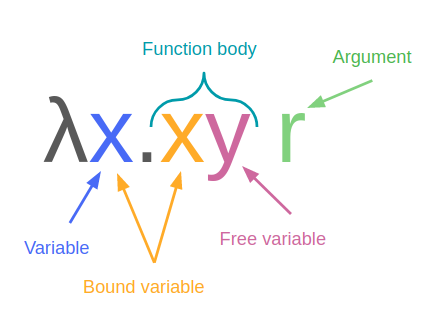
\includegraphics[scale=0.4]{lambdaCalculusFunctionExplenation.png}
    \caption{Visualization of the different parts of a lambda function}
    \label{fig:LC-explenations}
\end{figure}


\subsubsection{Lambda terms}
We have already explained how to build up terms above, but here we provide some extra information to understand terms better. Firstly, the \emph{abstraction} rule is the rule that defines the anonymous function. Secondly, the abstraction only forms the function and binds the variables; the abstraction does not execute the function. 

\subsubsection{Bound and Free variables}
As previously mentioned, the \emph{abstraction} sets the \emph{bound variables}. Within the abstraction, if the variable exists in the function body, the $\lambda$ binds this variable to the function body. For example, given the term $\lambda x.xy$, $x$ is a bound variable because: $x$ occurs in the function body, and $\lambda$ binds $x$ to the function body.

\para
\emph{Free variables} are the opposite of bound variables. Formally, we can say that if we have a term $E_1$ with a set $V_1$ for all variables and $B_1$ for bound variables; 
then the free variables $F_1$ are $F_1 = V_1\setminus B_1$. We can also extend this general rule further, 
by adding another term $E_1$ with a set $V_2$ for all variables and $B_2 $ for all the bound variables;
then the \emph{free variables} in $E_1 E_2$, $F_1 F_2$ equals $ (V_1\setminus B_1) \cup (V_2\setminus B_2)$. 
In other words, the set of free variables in the term $E_1 E_2$ is the union of the free variables in $E_1$ and $E_2$.

\subsubsection{$\alpha$-conversion}
To explain $\alpha$-conversion, one needs to understand what \emph{$\alpha$ equivalence} is. In short, two lambda terms are $\alpha$-equivalent if the only difference in the terms has the variables' names. E.g $\lambda ab.ab$ is alpha-equivalent to the lambda term $\lambda xy.xy$ 

\para
With $\alpha$-equivalent in mind, \emph{$\alpha$-conversion} is a way to change a variable name in both the $\lambda$ part and the function body while keeping the new term $alpha$ equivalent to the old term. E.g. $\alpha$-conversion of $\lambda ab.ab$ is $\lambda xy.xy$ since these are $alpha$ equivalent. Bear in mind that changing a variable name to an already existing variable name in the term is not allowed, because the result would change the meaning and thus the two terms would not be $alpha$ equivalent.

\para
As we have already mentioned, when doing $\alpha$-conversion, we can only change the names of the variables in the term so that the term does not change its meaning. 
E.g., $\lambda x.x \rightarrow_\alpha \lambda y.y$ since we have not changed the meaning of this term. The result of sending in any value/term $e$ will give us the same return value, in this case, just $e$ itself. An example of what is not allowed to do is this $\lambda x.xy \rightarrow_\alpha \lambda y.yy$, as these terms will give us different return values for an argument. Let us try with $e$ again; then we would see that  $\lambda x.xy e$ would give us $ey$ while $\lambda y.yy e$ would give us $ee$, and $ey \neq ee$. So the term $\lambda x.xy$ is $\alpha$-equivalent to all terms where we change to $x$ to anything except $y$. We can generally change any variable name to anything except the set of variables in the function body. Therefore $\lambda x.xy \rightarrow_\alpha \lambda z.zy$. Besides, we need to make sure that we only changes the variables that are in the same abstraction. So the term $\lambda x.\lambda x.x $ is not $\alpha$-equivalent to the 
term $\lambda y.\lambda x.y$, but to for example the terms $\lambda y.\lambda x.x$ or $\lambda x.\lambda y.y$.

\subsubsection{$\beta$-reduction}
$\beta$-reduction is a way to reduce terms. We reduce terms by sending in argument(s) for the bound variables. E.g., if we want to reduce the lambda term $\lambda x. x s$, 
we can $\lambda x. x$  $s \rightarrow _\beta s$ (this is the identity function, which gives us back the argument we gave to the function). We can do $\beta$-reduction in several rounds. When there are no more possible $\beta$-reductions, we say that the term has reached the $\beta$-normal form. \autoref{fig:beta-reduction} shows an example on $\beta$-reduction with a $\lambda$-term of one of the arguments. 

\para
If the term stays the same after one $\beta$-reduction, the term will never terminate. An example of a term that does not terminate while using $\beta$-reduction is the self-application function applied on itself $(\lambda f.ff) \lambda f.ff$.

\paragraph{Complexity}
$\beta$-reduction is not an atomic step; this means that one must locate all occurrences of a bound variable in a term, which can be very time-consuming. In O-notation, this will take $O(n)$ time for a term of length n. Also, storing all of these occurrences may become costly in regards to storage. 

\begin{figure}
    \centering
    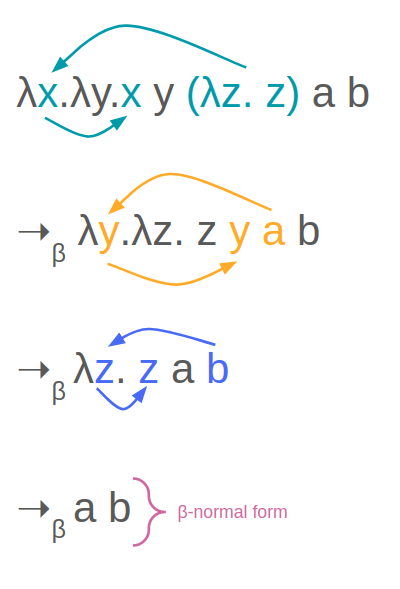
\includegraphics[scale=0.4]{b-reduction.png}
    \caption{An example of $\beta$-reduction}
    \label{fig:beta-reduction}
\end{figure}

\subsubsection{$\eta$-reduction}
$\eta$-reduction is the idea that two functions are equal if, and only if, they return the same result for any given argument. An example of $\eta$-reduction is $(\lambda x.f x)  \rightarrow_\eta f$, whenever $x$ is not a free variable in $f$.

\subsubsection{Combinatory logic}
Combinatory logic in computer science, is a theoretical method of computation. The idea is that we only have some base function to create new high-order functions. From now on, these functions will be called primitive functions. These primitive functions combined in the proper order can then express any other high-order function. Combinatory logic is often looked at as a variant of $\lambda$-calculus, where the lambda expressions are replaced with a limited set of primitive functions that does not have any free variables. 
The three primitive functions in combinatory logic is \textbf{I}, \textbf{K} and \textbf{S}.
\\ \\
Where \textbf{I} is the identity function, defined by: \\ 
\begin{center}
    $(I x) = x$\\    
\end{center}
Written in $\lambda$-calculus, the \textbf{I} function would look like this:\\
\begin{center}
    $\lambda x.x$\\    
\end{center}
Futhermore, we have the \textbf{K} function that takes in two arguments and always returns the first argument, defined by:
\begin{center}
    $ ((K x) y) = x$ or $(K x y) = x$\\    
\end{center}
Written in $\lambda$-calculus, the \textbf{K} function would look like this:\\
\begin{center}
    $\lambda xy.x$\\    
\end{center}
Lastly, we have the primitive function \textbf{S}, which takes in three arguments and applies the last argument on the two first arguments:
\begin{center}
    $ (S x y z) = (x z (y z))$\\    
\end{center}
Written in $\lambda$-calculus, the \textbf{S} function would look like this:\\
\begin{center}
    $\lambda xyz.xz(yz)$\\    
\end{center}
From these primitive functions and a variable $x$, we can build up combinatoric terms as shown in \autoref{tab:makeCombinatoricTerms} almost the same way that we build up different terms in $\lambda$-calculs. The difference between combinatoric logic and $\lambda$-calculus, is that we have a limited set of primitive functions in combinatoric logic, and in $\lambda$-calculus we have abstractions.

\begin{table}[]
    \centering
    \begin{tabular}{c c c | c}
         $E :=$&  & $x$ & (variable)\\
         & $|$ & $P$ & (the primitive functions) \\
         & $|$ & $E_1 E_1$ & (application, where $E_1$ and $E_2$ are combinatoric terms)\\
    \end{tabular}
    \caption{How to build up combinatoric terms}
    \label{tab:makeCombinatoricTerms}
\end{table}

\para
If we want to convert a lambda term to an equivalent combinator, we use a transformation $T[]$, which is defined by the following rules:
\begin{enumerate}
    \item $T[x] \Rightarrow x$
    \item $T[(E_1 E_2)] \Rightarrow (T[E_1]\; T[E_2])$
    \item $T[\lambda x.E] \Rightarrow (\textbf{K}\; T[E])$ (if x dosen't occure free in E)
    \item $T[\lambda x.x]\Rightarrow \textbf{I}$
    \item $T[\lambda x. \lambda y.E]\Rightarrow T[\lambda x.T[\lambda y.E]]$ (if x occures free in E)
    \item $T[\lambda x.(E_1 E_2)] \Rightarrow (\textbf{S} \; T[\lambda x.E_1] \; T[\lambda x.E_2])$
\end{enumerate}
T[] is not a well-typed mathematical function but a rewriter, which means that an uncompleted transformation will result in something that is neither a lambda term nor a combinatory term. 

\para
The following example explains how to transform the expression $\lambda x.\lambda y.xy$ from \autoref{fig:beta-reduction}. Note that we have made one shortcut to save time. The shortcut combines rule 3 and 1, which we write as $3/1$ in the example below.
In consequence, $T[\lambda x.y]$ we write $T[\lambda x.y] =_{3/1} (\textbf{K } y)$ instead of $T[\lambda x.y] =_{3} (\textbf{K } T[y]) =_{1} (\textbf{K } y)$.
\begin{quote}
    $\lambda x.\lambda y.xy$ \\
    $=_5 T[\lambda x.T[\lambda y.(xy)]]$ \\
    $=_6 T[\lambda x. (\textbf{S}\; T[\lambda y.x]\; T.[\lambda y.y])]$ \\
    $=_{3/1} T[\lambda x. (\textbf{S}\;(\textbf{K}\; x) \; T.[\lambda y.y])]$ \\  
    $=_4 T[\lambda x. (\textbf{S}\;(\textbf{K}\; x) \; \textbf{I})]$ \\
    $=_6 (\textbf{S} \; T.[\lambda x.(\textbf{S}\;(\textbf{K}\; x))] \; T.[\lambda x.I])$ \\
    $=_{3/1} (\textbf{S} \; T.[\lambda x.(\textbf{S}\;(\textbf{K}\; x))] \; (\textbf{K I}))$ \\
    $=_{6} (\textbf{S} \; (\textbf{S} \; T[\lambda x.\textbf{S}] \; T[\lambda x.(\textbf{K} \; x)]) \; (\textbf{K I}))$ \\
    $=_{3/1} (\textbf{S} \; (\textbf{S} \; (\textbf{K S}) \; T[\lambda x.(\textbf{K} \; x)]) \; (\textbf{K I}))$ \\
    $=_{6} (\textbf{S} \; (\textbf{S} \; (\textbf{K S}) \; (\textbf{S} \; T.[\lambda x.\textbf{K}] \; T.[\lambda x.\textbf{x}]) ) \; (\textbf{K I}))$ \\
    $=_{3/1} (\textbf{S} \; (\textbf{S} \; (\textbf{K S}) \; (\textbf{S} \; (\textbf{K K}) \; T.[\lambda x.\textbf{x}]) ) \; (\textbf{K I}))$ \\
    $=_4 (\textbf{S} \; (\textbf{S} \; (\textbf{K S}) \; (\textbf{S} \; (\textbf{K K}) \; \textbf{I}) ) \; (\textbf{K I}))$ \\      
\end{quote}
It is common to add the combinatory terms \textbf{B} ($(\textbf{C} f g x) = ((f x )g)$) 
and \textbf{C} ($(\textbf{C} f g x) = (f (x g))$). \textbf{C} performes substitution on the the first term, and \textbf{B} on the second term, in contrast to \textbf{S} which performs substitution on both terms. These two terms can now be added to the transformation, $T[]$:
\begin{enumerate}
    \setcounter{enumi}{6}
    \item $T[\lambda x.(E_1 E_2)] \Rightarrow (\textbf{C} \; T[\lambda x.E_1] \; T[E_2]))$ (if x is free in $E_1$ but not in $E_2$)
    \item $T[\lambda x.(E_1 E_2)] \Rightarrow (\textbf{B} \; T[E_1] \; T[\lambda x.E_2])$ (if x is free in $E_2$ but not in $E_1$)
\end{enumerate}
\textbf{B} and \textbf{C} are define as the following using the primitive functions:\\
$\textbf{B=(S(K S)K)}$\\
$\textbf{C=(S(S(K(S(K S)K))S)(K K))}$\\

\subsection{Type theory}
Type theory is the academic study of \emph{type systems}, which gives every term a type. The type determines the meaning, and which operations are possible to perform on a term. Lambda Calculus has its own type system, also made by Alonzo Church called \emph{Simply Typed Lambda Calculus}, which we discuss in \autoref{Simply Typed Lambda Calculus}.

\para
\emph{A term} is often followed by a : and then the type of the term. \emph{A type} in a type system is semantically a collection of different values that a term can be evaluated to be. Therefore, there are many similarities between type systems and set theory, although they have their differences. Furthermore, the name of a given term is syntactic. For example, in java, where we have a type that is a collection of all Integers ($\mathbb{Z}$) (semantic) and has the name int (syntactic). Consequently, a term $e$ ($e$ is often used to denote a term) is of type $\tau$ ($\tau$ is often used to denote a type) if $e \in \tau$. E.g. 2 is of type $\mathbb{N}$ (natural numbers) because $2 \in \mathbb{N}$. Making new types depends on the type systems' set of base types and type constructors, often called the \emph{inductive types} of a type system. An example type system with the base type $\sigma$, two type constructors $*$ and $\#$, and two types $M$ and $N$, makes it possible to make a new type $T$ as shown in \autoref{tab:inductive types}. 

\para
Many of the programming languages using type systems either require that all expressions terminate (e.g. Coq) or allow infinite loops but are inconsistent when viewed as logics (e.g. Haskel) \textbf{(src: http://www.tyconmismatch.com/papers/combining-TR.pdf)}.
Therefore in some programming languages like \nameref{Simply Typed Lambda Calculus}, one of the type systems goals is to make sure that a term terminates. 

\begin{table}[]
    \centering
    \begin{tabular}{c c c}
         $T :=$&  & $\sigma$\\
         & $|$ & $M * N$ \\
         & $|$ & $M \# N$ \\
    \end{tabular}
    \caption{Example of how to build up inductive types}
    \label{tab:inductive types}
\end{table}


\subsubsection{Decision problems}
Type theory uses type checking, typability and type inhabitation as decisions problems. These decision problems uses judgments, which are denoted with $\Upgamma \vdash e:\tau$. Where $\Upgamma$ is the denotation which is usually used for a context or environment. A terms' type is determined using the judgment and equivalences type inference rules. 

\para
The decision problem of \textbf{checking} (abbreviated by ($\Upgamma\vdash e : \tau$?) is:\\
\textit{Given a type environment $\Upgamma$, a term $e$, and a type $\tau$, decide whether the term $e$ can be assigned the type $\tau$ in the type environment $\Upgamma$} \\ \\
The decision problem of type \textbf{typability} (abbreviated by ($ \exists \Upgamma,\tau .\Upgamma\vdash e : \tau$?) is: \\ 
\textit{Given  a term $e$, decide wheter there exists a type environment $\Upgamma$ and a type $\tau$ such that the term $e$ can be assigned the type $\tau$ in the type environment $\Upgamma$} \\ \\ 
The decision problem of type \textbf{inhabitation} (abbreviated by ($ \exists e.\Upgamma \vdash e : \tau$?) is: \\
\textit{Given a type environment $\Upgamma$ and a type $\tau$, decide whether there exists a term $e$ that can be assigned the type $\tau$ in the type environment $\Upgamma$}

\subsection{Simply Typed Lambda Calculus}
\label{Simply Typed Lambda Calculus}
As earlier mention, Simply Typed Lambda Calculus 
($\lambda^\rightarrow$) is a Type Theory developed by Alonzo Church for $\lambda$-calculus. \\ \\
In $\lambda^\rightarrow$, we can make types with only one operator $\rightarrow$ and a set of base types,
 often denoted with $B$. From the base types, $B$, we can construct new types using the constructor 
 $\rightarrow$. The result of a type system having the two base types $\tau$ and $\sigma$ is that the type system can construct a new type $\tau \rightarrow \sigma$. This type would refer to a function that takes in an argument of type $\tau$ and returns a term of type $\sigma$. \\ \\
The syntax for $\lambda^\rightarrow$ are more or less equal to \nameref{Lambda Calculus}s syntax, except that we need to specify the type of a variable in the function (in the abstraction).
The specification is done in the way described in \nameref{Type Theory} with $x:\tau$ for a variable $x$ with type $\tau$. Furthermore, Simply typed lambda calculus also adds term constant, often denoted with a $c$. The full syntax for 
Simply Typed Lambda Calculus is shown in the table \nameref{tab:STLC syntax} \\

\begin{table}[]
    \centering
    \begin{tabular}{c c c}
         $e :=$&  & $x$\\
         & $|$ & $\lambda x:\tau.M$ \\
         & $|$ &  $M N$ \\
         & $|$ &  $c$ \\
    \end{tabular}
    \caption{Simply Typed Lambda Calculus syntax}
    \label{tab:STLC syntax}
\end{table}

\subsubsection{Typing rules}
In Simply Typed Lambda Calculus, we have four typing rules. 
To state these rules, we need to use the typing environment described in the section about \nameref{Type Theory}.

\begin{enumerate}
    \item If we have variable $x$ that is of type $\tau$ in the typing environment $\Upgamma$, then we know that $x$ has type $\tau$.
    \item If we have a constant $c$ of type $T$ in the typing environment $\Upgamma$, then we know that $c$ has type $T$.
    \item If we have a variable $x$ that is of type $\tau$ in a type environment, and with a term $e$ of type $\sigma$ in the same type environment, then we have a term $\lambda x\tau .e$ with the type $\tau \rightarrow \sigma$ in the same type environment.
    \item If we have a term $M$ of type $\tau \rightarrow \sigma$ and a term $N$ of type $\tau$ in an typing environment, then $M N$ will have the type $\sigma$ in the same typing environment.
\end{enumerate}

\subsubsection{Reduction of Simply Typed Lambda Calculus}
Simply Typed Lambda Calculus also uses the $\beta$-reduction and $\eta$-reduction as mention in the section about \nameref{Lambda Calculus}. 
Additional, the reduction needs to check that the arguments to the function have 
the right type in typing environment as well. 
\\ \\
To give an example of $\beta$-reduction, we first need to make a set of the base types. In this case, we will only use $Int$, the collection of all-natural numbers. 
From $Int$, it is possible to make an unlimited set of types ($Int, Int \rightarrow Int, Int \rightarrow Int \rightarrow Int$ etc).
For the sake of this example, we will add the operation $+$ that adds to numbers together.
We will use the term $e_1:= \lambda x:Int\: y:Int. + x y:Int \rightarrow Int \rightarrow Int$. The type $Int \rightarrow Int \rightarrow Int$ in writing would be "a term
which takes in an Int and returns a term which takes in an Int and returns an Int". 
Applying $e_2 := 3:Int$ with the third typing rule on 
the term $e_1$, $e_1 e_2$ will result in the term  
$e_1 e_2$ with the type $Int \rightarrow Int$ (taking in a Int and returning a Int). This can be proved using $\beta$-reduction on the term:
\\ \\
$e_1 e_2 := \lambda x:Int\: y:Int. + x y:Int \rightarrow Int \rightarrow Int\; 3:Int 
\newline\rightarrow_\beta \lambda y:Int. + 3\; y: Int \rightarrow Int$
\\ \\
Using the third typing rule again, applying 
$e_3 := 7:Int$ on the term $e_1 e_2:Int \rightarrow Int$ will result in the term $e_1 e_2 e_3$ with the type $Int$.
The $\beta$ reduction also proves this: 
\\ \\
$e_1 e_2 e_3 := \lambda y:Int. + 3\; y: Int \rightarrow Int \; 7:Int
\newline \rightarrow_\beta + 3:int \; 7:Int = 10$

\subsection{Evaluation strategies}
An \textit{evaluation strategy} is a strategy used in programming languages to decide when a programming language should evaluate an expression. 
Meaning that the evaluation strategy, for example, chooses whether the programming language evaluates the arguments of a function before it is called or 
if the whole expression is sent in to be evaluated at a later stage. Evaluation strategy has two main strategies \textbf{eager evaluation} (strict evaluation) 
and \textbf{non-strict evaluation}. To briefly explain, eager evaluation will evaluate the expression as soon as it is bound. 
One of the main differences between eager evaluation and non-strict evaluation is that eager evaluation, on the one hand, 
would evaluate every argument before the function call. While in non-strict evaluation, on the other hand, 
the programming language evaluates the expression when it is used. 
Meaning that eager evaluation will evaluate the arguments of a function, although the arguments may never be used. 
Non-strict evaluation can also have an infinite list, also called streams, since only the element in the list which is used are calculated. 
One negative aspect of non-strict evaluation is that an expression used $n$ times will end up being evaluated $n$ times. 
\\ \\
Most Imperative programming languages use an eager evaluation. The reason why eager evaluation is the most practised evaluation strategies in 
imperative programming languages is that it is easier to avoid unexpected behaviour. Additional to being easier to debug compared to non-strict evaluation. 
One can also have some difficulties using imperative features like I/O and exception handling when using a non-strict evaluation strategy. 
Although most imperative languages use eager evaluation, they often utilise some non-strict evaluation methods. A good example of this is the if-statement, 
where most languages only will evaluate the part of the if-statement that is true. The pseudo-code $if\; a\; then\; b\; else\; c$, will only evaluate b if a is evaluates to be true. 
c, on the other hand, will only be evaluated if a is false. However, if the if-statement is put in a function and use $a$ $b$ and $c$ as arguments 
like this $f(a, b,c):= \; if\; a\; then\; b\; else\; c$ then eager evaluation will evaluate all the expressions before the functions start. 
Despite that, the programming language only needs to evaluate either $b$ or $c$. While non-strict evaluation, on the other hand,  only evaluates the used expressions.
\\ \\
\textbf{Lazy evaluation} (also know as call-by-need) is a type of non-strict evaluation that Functional programming often uses. Since Lazy evaluation is a type of non-strict evaluation, 
it evaluates the expression when it is used. What separating lazy evaluation from the other types of non-strict evaluation, such as call-by-name,
is that Lazy evaluation also uses memorisation to avoid repeated evaluations, reducing the running time. Memorisation uses a look-up table where the evaluated value of a function for some given arguments is stored. 
When the evaluation is executed on an expression, lazy evaluation first checks if it already exists in the look-up table. If the value exists, 
it is retrieved from the table. However, if the value is not in the look-up table, lazy evaluation evaluates the function to a value and appends this value to the table.
\textbf{Graph reductuion} is an efficient technique for implementing lazy evaluation using the outermost tree reduction method.
\\ \\
Figure \nameref{fig:strictVSLazy} is  an example of strict evaluation and lazy evaluation with $\beta$-reduction. Assuming that print is a term that prints the argument to the terminal 
and that + - and * are operators that work on integers. Some differences are important to note:

\begin{itemize}
    \item Strict evaluation will evaluate an expression(terms) as soon as it is bound. While lazy evaluation waits until the expression is used.
    \item Strict evaluation evaluates the expressions(terms) before sending them in, while we in lazy evaluation send in the whole expression ref. $(\lambda x.\lambda y. - x y)\; 4 \; 2$. Since the $y$ is not used anywhere in the function body, the result is that strict evaluation ends up evaluating something that never is used.
    \item On the last two lines, lazy evaluation uses memorisation and the look-up table to retrieve the return value instead of evaluating it.
\end{itemize}


\begin{figure}
    \centering
    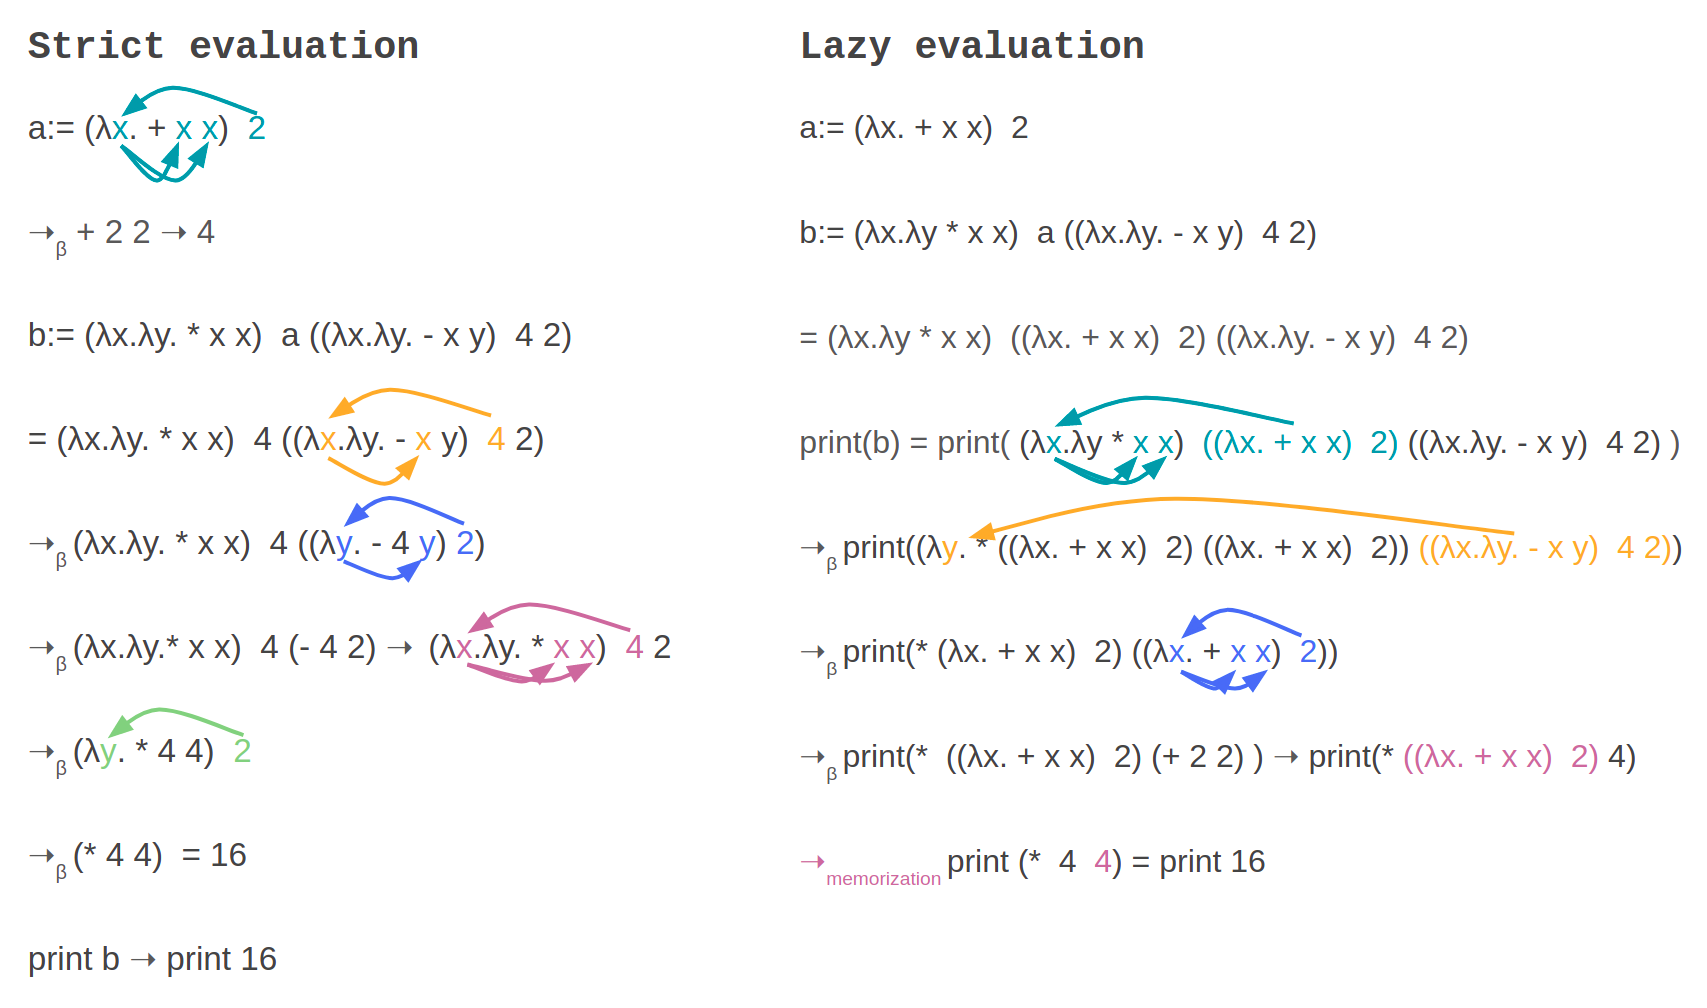
\includegraphics[scale=0.25]{strictVSLazy.png}
    \caption{Shows the difference between strict evaluation and lazy evaluation. Here we assume that print is a term which 
    prints the argument to the terminal, and that + - and * are operators that work on integers}
    \label{fig:strictVSLazy}
\end{figure}

\subsection{Undecided title (Practical use of functional programming)}
Several of the theoretical foundations mention earlier
influence how the different functional programming languages (and non-functional language, for that matter) are built up.
\\ \\
Functional programming is a programming paradigm that is made by applying and composing functions. Furthermore, 
functional programming is inspired by a combination of \nameref{Lambda Calculus}, types and definitions. We see \nameref{Lambda Calculus} different impacts in several
of the concepts in functional programming. 
First off, functional programming uses high-order functions, which are functions that can take in functions as arguments
and return a function. In other words, functional programming allows functions to be both an argument and a return value of a function. 
The use of high-order functions is something that we see in lambda calculus as well. Some well known high-order functions are map 
(which takes in a function taking in one argument and a list and applies the function on every element, returning 
a new list with every element in the original list mapped), 
filter(which takes in a function with one argument and a list and applies it to each element of the list, the function should return a boolean and returns a new list with only the elements
that returned true in the function), and reduce also called fold (which recursively applies the function given as the first argument to the next ones). 
The use of high-order functions in functional programming enables partial application or currying. Partial application or currying is a technique
where every argument to a function is applied simultaneously, from the first one to the last one. 
\\ \\
From the 70s, functional programming started to add type systems in their programming languages,
using typed lambda calculus, where \nameref{Simply Typed Lambda Calculus} is a type of typed lambda calculus. 
The reason for using typed lambda calculus is that it makes the program more reliable because it enables improved compile-time type checking.  
\\ \\
Two other important concepts in functional programming are Pure function and recursion. Pure functions are a function without any side effects. 
Meaning that the programming language, among other things, can assure that a function always will return the same answers as long as the arguments have no side effects. A programming language that does not allow 
side effects make it more optimal to use memorization because we know that a function is given to an argument always will yield the same answer 
making it suitable for an evaluation strategy like Lazy evaluation.